\documentclass[../main.tex]{subfiles}

\begin{document}
	
A continuación introduciremos el concepto de hipercategoría y, siguiendo el camino trazado en el capítulo anterior, veremos los lenguajes que generan estos objetos para luego notar que hemos avanzado en la jerarquía de Chomsky, ya que estos son precisamente los lenguajes libres de contexto, o de tipo $0$. Finalmente, implementaremos estos conceptos en \texttt{Python}.

\section{Hipercategorías}

\begin{dfn}
	Una \textbf{signatura de hipercategoría} es un conjunto de nodos $H_1$ y uno de objetos \(H_0\) junto a un par de funciones
	\[
		H_0^* \xleftarrow{dom} H_1 \xrightarrow{cod} H_0
	\] 
	
	Un morfismo de signaturas de hipercategorías $\varphi : H \to \Gamma$ es un par de funciones $\varphi_0 : H_0 \to \Gamma_0$ y $\varphi_1 : H_1 \to \Gamma_1$ tal que el siguiente diagrama conmuta: 
	
	\[
	\begin{tikzcd}
		H_0^* \arrow{d}{\phi_0} & H_1 \arrow{r}{\tt{dom}} \arrow{l}{\tt{cod}} \arrow{d}{\phi_1} & H_1 \arrow{d}{\phi_0} \\
		\Gamma_0^* & \Gamma_1 \arrow{r}{\tt{dom}} \arrow{l}{\tt{cod}} & \Gamma_1
	\end{tikzcd}
	\]
	Con tales morfismos, las signaturas de hipergráficas forman la categoría \textbf{HypCat}.
\end{dfn}
	
Dado una signatura de hipergráfica, denotaremos un nodo $b_1...b_n \xrightarrow{f} a$ graficamente como: 
	
	\begin{center}
	\begin{tikzpicture}[node distance={10mm}, thick, main/.style = {draw, circle, fill=black, inner sep=0pt, minimum width=2pt},
		letter/.style={circle,draw=white,very thick}] 
		
		\node[main] (1) {};
		\node[letter] (2) [right of=1] {$\cdots$};
		\node[main] (3) [right of=2]{};
		\node[main] (4) [below of=2]{};
		\node[main] (5) [below of=4]{};
		
		\draw[-] (1) -- (4);
		\draw[-] (3) -- (4);
		\draw[-] (4) -- (5);
		
		\node[letter] (p) at (-0.5,0) {$b_1$};
		\node[letter] (p) at (2.5,0) {$b_n$};
		\node[letter] (p) at (1.5,-1) {$f$};
		\node[letter] (p) at (1.5,-2) {$a$};
	\end{tikzpicture}
	\end{center}

Además, diremos que $f$ tiene aridad $n$.

\begin{ej}
	Consideremos la siguiente signatura de hipergráfica donde los objetos corresponderán a los números reales, $\mathbb{R}$. Luego, dado $a, ab \in \mathbb{R}^*$ tenemos los siguientes nodos: 
	\begin{multicols}{4}
			\begin{center}
			\begin{tikzpicture}[node distance={10mm}, thick, main/.style = {draw, circle, fill=black, inner sep=0pt, minimum width=2pt},
				letter/.style={circle,draw=white,very thick}] 
				
				\node[main] (1) {};
				\node[main] (4) (p) at (0,-2){};
				
				\draw[-] (1) to (0,-2);
				
				\node[letter] (p) at (-0.5,0) {$a$};
				\node[letter] (p) at (-0.5,-2) {$a$};
			\end{tikzpicture}
		\end{center}
		
			\begin{center}
				\begin{tikzpicture}[node distance={10mm}, thick, main/.style = {draw, circle, fill=black, inner sep=0pt, minimum width=2pt},
					letter/.style={circle,draw=white,very thick}] 
					
					\node[main] (1) {};
					\node[main] (4) (p) at (0,-2){};
					
					\draw[-] (1) to (0,-2);
					
					\node[letter] (p) at (-0.5,0) {$a$};
					\node[letter] (p) at (-0.5,-2) {$-a$};
				\end{tikzpicture}
			\end{center}
		
			\begin{center}
			\begin{tikzpicture}[node distance={10mm}, thick, main/.style = {draw, circle, fill=black, inner sep=0pt, minimum width=2pt},
				letter/.style={circle,draw=white,very thick}] 
				
				\node[main] (1) {};
				\node[main] (2) (p) at (1.5, 0) {};
				\node[main] (3) (p) at (.75, -1) {};
				\node[main] (4) (p) at (.75, -2) {};

				
				\draw[-] (1) to (.75, -1);
				\draw[-] (1.5, 0) to (.75, -1);
				\draw[-] (.75,-1) to (.75, -2);
				
				\node[letter] (p) at (-.5,0) {$a$};
				\node[letter] (p) at (2,0) {$b$};
				\node[letter] (p) at (1.35,-2) {$a+b$};
				
			\end{tikzpicture}
			\end{center}
		
			\begin{center}
				\begin{tikzpicture}[node distance={10mm}, thick, main/.style = {draw, circle, fill=black, inner sep=0pt, minimum width=2pt},
					letter/.style={circle,draw=white,very thick}] 
					
					\node[main] (1) {};
					\node[main] (2) (p) at (1.5, 0) {};
					\node[main] (3) (p) at (.75, -1) {};
					\node[main] (4) (p) at (.75, -2) {};
					
					
					\draw[-] (1) to (.75, -1);
					\draw[-] (1.5, 0) to (.75, -1);
					\draw[-] (.75,-1) to (.75, -2);
					
					\node[letter] (p) at (-.5,0) {$a$};
					\node[letter] (p) at (2,0) {$b$};
					\node[letter] (p) at (1.35,-2) {$a\cdot b$};
					
				\end{tikzpicture}
			\end{center}
	\end{multicols}
	Notemos que los primeros dos nodos corresponden a las operaciones de aridad $1$ que lleva un número asímismo o a su inverso aditivo, respectivamente. Por otro lado, los últimos dos nodos corresponden a las operaciones binarias usuales de los números reales: la adición y la multiplicación. \\
	Notemos, además, que para cualquier $abc \in \mathbb{R}^*$ tenemos que, dado que nuestras operaciones son asociativas, entonces $a+(b+c)=(a+b)+c$, así gráficamente tenemos la igualdad de los siguientes diagramas:
	
	\begin{center}
	\begin{tikzpicture}[node distance={10mm}, thick, main/.style = {draw, circle, fill=black, inner sep=0pt, minimum width=2pt},
		letter/.style={circle,draw=white,very thick}] 
		
		\node[main] (1) {};
		\node[main] (p) at (1,2) {};
		\node[main] (p) at (2,1) {};
		\node[main] (p) at (3,2) {};
		\node[main] (p) at (2,0) {};
		\node[main] (p) at (1,-1) {};
		\node[main] (p) at (1,-2) {};
		
		\node[main] (p) at (5,2) {};
		\node[main] (p) at (6,1) {};
		\node[main] (p) at (7,2) {};
		\node[main] (p) at (6,0) {};
		\node[main] (p) at (8,0) {};
		\node[main] (p) at (7,-1) {};
		\node[main] (p) at (7,-2) {};
		
		\draw[-] (1,2) to (2,1);
		\draw[-] (3,2) to (2,1);
		\draw[-] (2,1) to (2,0);
		\draw[-] (0,0) to (1,-1);
		\draw[-] (2,0) to (1,-1);
		\draw[-] (1,-1) to (1,-2);
		
		\draw[-] (5,2) to (6,1);
		\draw[-] (7,2) to (6,1);
		\draw[-] (6,1) to (6,0);
		\draw[-] (6,0) to (7,-1);
		\draw[-] (8,0) to (7,-1);
		\draw[-] (7,-1) to (7,-2);
		
		\node[letter] (p) at (4,0) {$=$};
	
		
	\end{tikzpicture}
	
	\end{center}
	
	Por ello, siguiendo un razonamiento inductivo para cualesquiera $a_1\dots a_n\in \mathbb{R}$ podemos agregar los nodos: 
	
	\begin{multicols}{2}
	
	\begin{center}
		\begin{tikzpicture}[node distance={10mm}, thick, main/.style = {draw, circle, fill=black, inner sep=0pt, minimum width=2pt},
			letter/.style={circle,draw=white,very thick}] 
			
			\node[main] (1) {};
			\node[letter] (2) [right of=1] {$\cdots$};
			\node[main] (3) [right of=2]{};
			\node[main] (4) [below of=2]{};
			\node[main] (5) [below of=4]{};
			
			\draw[-] (1) -- (4);
			\draw[-] (3) -- (4);
			\draw[-] (4) -- (5);
			
			\node[letter] (p) at (-0.5,0) {$a_1$};
			\node[letter] (p) at (2.5,0) {$a_n$};
			\node[letter] (p) at (2.5,-2) {$a_1 + \cdots + a_n$};
		\end{tikzpicture}
	\end{center}
	
	\begin{center}
		\begin{tikzpicture}[node distance={10mm}, thick, main/.style = {draw, circle, fill=black, inner sep=0pt, minimum width=2pt},
			letter/.style={circle,draw=white,very thick}] 
			
			\node[main] (1) {};
			\node[letter] (2) [right of=1] {$\cdots$};
			\node[main] (3) [right of=2]{};
			\node[main] (4) [below of=2]{};
			\node[main] (5) [below of=4]{};
			
			\draw[-] (1) -- (4);
			\draw[-] (3) -- (4);
			\draw[-] (4) -- (5);
			
			\node[letter] (p) at (-0.5,0) {$a_1$};
			\node[letter] (p) at (2.5,0) {$a_n$};
			\node[letter] (p) at (2,-2) {$a_1 \cdots a_n$};
		\end{tikzpicture}
	\end{center}
	
	\end{multicols}
	Así, todos los nodos son los representados por alguno de los diagramas anteriores. Con lo anterior, tenemos una signatura de hipercategoría. 
\end{ej}

Ahora, veamos la definición principal de esta sección: 

\begin{dfn}
	Un \textbf{hipercategoría} es una signatura de hipercategoría \textbf{H} junto a una operación de composición \( \Pi_{b_i \in \vec{b}} \textbf{Hyp} (\vec{c_i}, b_i) \times \textbf{Hyp} (\vec{b}, a) \to \textbf{Hyp} (\vec{c}, a) \) con $a \in \textbf{O}_0$ y $\vec{c}, \vec{b} \in \textbf{O}_0^*$. Dadas  $f: \vec{b} \to a$  y $g_i : \vec{c_i} \to b_i$ definimos la composición como:
	\[
		(c_1^1, c_2^1, \dots , c_{m_1}^1, c_2^1, \dots , c_1^n, \dots , c_{m_n}^n) \mapsto f(g_1(c_1^1, \dots , c_{m_1}^1), \dots , g_n(c_1^n, \dots , c_{m_n}^n) )	
	\] 
	que representamos gráficamente de la siguiente manera 
	
	\begin{center}
		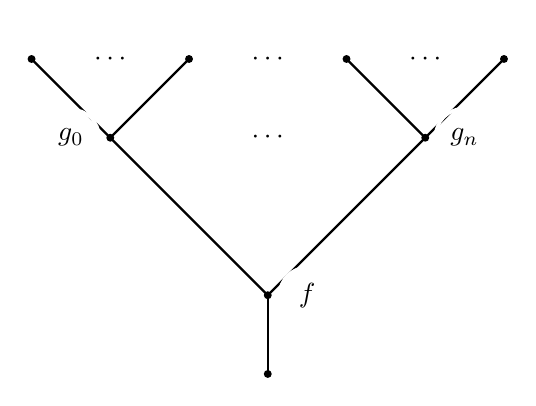
\begin{tikzpicture}[node distance={10mm}, thick, main/.style = {draw, circle, fill=black, inner sep=0pt, minimum width=2pt},
			letter/.style={circle,draw=white,very thick}] 
			
			\node[main] (1) {};
			\node[main] (p) at (2,0) {};
			\node[main] (p) at (4,0) {};
			\node[main] (p) at (6,0) {};
			\node[main] (p) at (1,-1) {};
			\node[main] (p) at (5,-1) {};
			\node[main] (p) at (3,-3) {};
			\node[main] (p) at (3,-4) {};
			
			\draw[-] (0,0) to (1,-1);
			\draw[-] (2,0) to (1,-1);
			\draw[-] (4,0) to (5,-1);
			\draw[-] (6,0) to (5,-1);
			\draw[-] (1,-1) to (3,-3);
			\draw[-] (5,-1) to (3,-3);
			\draw[-] (3,-3) to (3,-4);
			
			\node[letter] (p) at (1,0) {$\cdots$};
			\node[letter] (p) at (3,0) {$\cdots$};
			\node[letter] (p) at (5,0) {$\cdots$};
			\node[letter] (p) at (3,-1) {$\cdots$};
			\node[letter] (p) at (.5,-1) {$g_0$};
			\node[letter] (p) at (5.5,-1) {$g_n$};
			\node[letter] (p) at (3.5,-3) {$f$};
			
		\end{tikzpicture}
	\end{center}
	
	Además, para cualquier $a \in \textbf{H}_0$ tenemos una identidad $a \xrightarrow{Id_a} a$ en donde se satisfacen las siguientes propiedades:
	
	\begin{enumerate}
		\item Para cualquier $f:\vec{b} \to a$ en $\textbf{O}_1$, $f \cdot Id_a = f = \vec{Id}_{b_i} \cdot f$; y 
		\item Para cualesquiera $f: \vec{b} \to a$  y $g_i : \vec{c_i} \to b_i$ tenemos que: 
		
	\begin{center}
	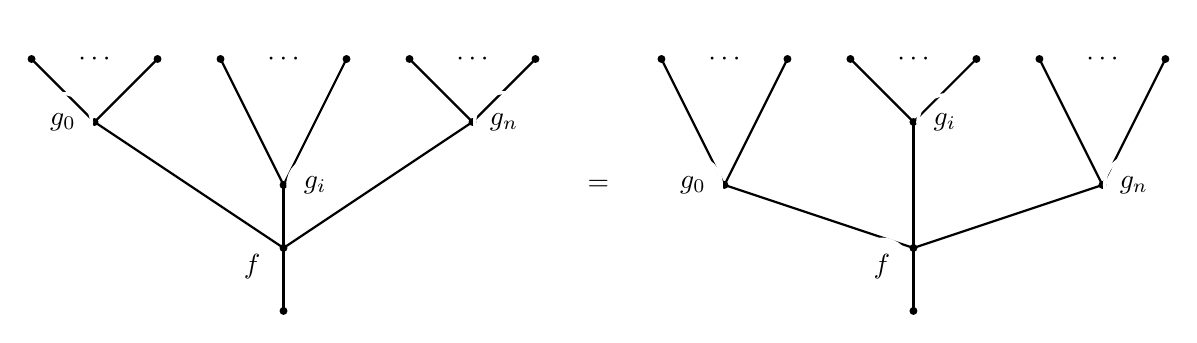
\begin{tikzpicture}[scale=0.8, node distance={10mm}, thick, main/.style = {draw, circle, fill=black, inner sep=0pt, minimum width=2pt},
		letter/.style={circle,draw=white,very thick}] 
		
		\node[main] (1) {};
		\node[main] (p) at (2,0) {};
		\node[main] (p) at (3,0) {};
		\node[main] (p) at (5,0) {};
		\node[main] (p) at (6,0) {};
		\node[main] (p) at (8,0) {};
		\node[main] (p) at (1,-1) {};
		\node[main] (p) at (7,-1) {};
		\node[main] (p) at (4,-2) {};
		\node[main] (p) at (4,-3) {};
		\node[main] (p) at (4,-4) {};
		
		\draw[-] (0,0) to (1,-1);
		\draw[-] (2,0) to (1,-1);
		\draw[-] (3,0) to (4,-2);
		\draw[-] (5,0) to (4,-2);
		\draw[-] (6,0) to (7,-1);
		\draw[-] (8,0) to (7,-1);
		\draw[-] (1,-1) to (4,-3);
		\draw[-] (7,-1) to (4,-3);
		\draw[-] (4,-3) to (4,-4);
		\draw[-] (4,-2) to (4,-3);
		
		\node[letter] (p) at (1,0) {$\cdots$};
		\node[letter] (p) at (4,0) {$\cdots$};
		\node[letter] (p) at (7,0) {$\cdots$};

		\node[letter] (p) at (.5,-1) {$g_0$};
		\node[letter] (p) at (4.5,-2) {$g_i$};
		\node[letter] (p) at (7.5,-1) {$g_n$};
		\node[letter] (p) at (3.5,-3.3) {$f$};
		
		\node[letter] (p) at (9,-2) {$=$};
		
		\node[main] (p) at (10,0) {};
		\node[main] (p) at (12,0) {};
		\node[main] (p) at (13,0) {};
		\node[main] (p) at (15,0) {};
		\node[main] (p) at (16,0) {};
		\node[main] (p) at (18,0) {};
		\node[main] (p) at (11,-2) {};
		\node[main] (p) at (14,-1) {};
		\node[main] (p) at (17,-2) {};
		\node[main] (p) at (14,-3) {};
		\node[main] (p) at (14,-4) {};
		
		\draw[-] (10,0) to (11,-2);
		\draw[-] (12,0) to (11,-2);
		\draw[-] (13,0) to (14,-1);
		\draw[-] (15,0) to (14,-1);
		\draw[-] (16,0) to (17,-2);
		\draw[-] (18,0) to (17,-2);
		\draw[-] (11,-2) to (14,-3);
		\draw[-] (17,-2) to (14,-3);
		\draw[-] (14,-1) to (14,-4);
		\draw[-] (14,-2) to (14,-3);
		
		\node[letter] (p) at (11,0) {$\cdots$};
		\node[letter] (p) at (14,0) {$\cdots$};
		\node[letter] (p) at (17,0) {$\cdots$};
		
		\node[letter] (p) at (10.5,-2) {$g_0$};
		\node[letter] (p) at (14.5,-1) {$g_i$};
		\node[letter] (p) at (17.5,-2) {$g_n$};
		\node[letter] (p) at (13.5,-3.3) {$f$};
		
	\end{tikzpicture}
	\end{center}
		
		
		
	\end{enumerate} 
	
	Un álgebra $F: \textbf{H} \to \textbf{N}$ es un morfismo de signatura de hipercategorías compatible con la composición, es decir, cada que $\vec{c} \xrightarrow{\vec{g}} \vec{b} \xrightarrow{f} a$, $F(\vec{g} \cdot f) = F(\vec{g}) \cdot F(f)$ 
	
\end{dfn}

Es importante resaltar que la propiedad $2$ nos indica que no importa el orden en que hagamos las composiciones, es decir, se respeta cierta noción de asociatividad. Vale la pena resaltar que todavía no definimos formalmente el significado del cálculo de diagramas presentado, pues lo analizaremos con detenimiento en el siguiente capítulo. \\ 
Notemos que la signatura de hipercategoría del ejemplo anterior es propiamente un hipercategoría con la composición dada de la manera obvia. \\


De manera análoga al capítulo anterior, nuestra intención es definir una hipercategoría libre. Antes, veamos la siguiente definición: 

\begin{dfn}
	Sea \textbf{H} una hipergráfica. Sea $f:\vec{b} \to a$ y $g: \vec{c} \to b_i$ en $\textbf{H}_1$ con $i \in \{1, ..., n\}$ con $n$ es la aridad de $f$. \\
	Definimos la composición parcial en la $i-$ésima entrada como: 
	\[
		g \circ_i f = (id_{b_1}\cdots g\cdots id_{b_n})\cdot f 
	\]
	Graficamente
	
	\begin{center}
		\begin{tikzpicture}[node distance={10mm}, thick, main/.style = {draw, circle, fill=black, inner sep=0pt, minimum width=2pt},
			letter/.style={circle,draw=white,very thick}] 
			
			\node[main] (1) {};
			\node[main] (p) at (2,0) {};
			\node[main] (p) at (4,0) {};
			\node[main] (p) at (6,0) {};
			
			\node[main] (p) at (0,-1) {};
			\node[main] (p) at (6,-1) {};
			\node[main] (p) at (3,-1) {};
			
			\node[main] (p) at (3,-2) {};
			
			\draw[-] (0,0) to (0,-1);
			\draw[-] (2,0) to (3,-1);
			\draw[-] (4,0) to (3,-1);
			\draw[-] (6,0) to (6,-1);
			\draw[-] (6,-1) to (3,-2);
			\draw[-] (0,-1) to (3,-2);
			\draw[-] (3,-1) to (3,-2);
			\draw[-] (3,-2) to (3,-3);
			
			\node[letter] (p) at (1,0) {$\cdots$};
			\node[letter] (p) at (3,0) {$\cdots$};
			\node[letter] (p) at (5,0) {$\cdots$};

			\node[letter] (p) at (-.5,-1) {$Id_{b_1}$};
			\node[letter] (p) at (6.5,-1) {$Id_{b_n}$};
			\node[letter] (p) at (3.5,-1.2) {$g$};
			\node[letter] (p) at (3.5,-2.3) {$f$};
			
		\end{tikzpicture}
	\end{center}
	
	
\end{dfn}

Una observación importante es que definimos la composición parcial a partir de la composición, pero también pudimos definirlo inversamente de la siguiente forma: 
\[
	[g_1\cdots g_n] \cdot f = g_{n}\circ_{n}(g_{n-1}\circ_{n-1}\dots \circ _2(g_1 \circ_1 f)...)
\]
Notemos que la propiedad $2$ de la composición para hipergráficas nos garantiza que efectivamente la composición anterior coincide con la usual. \\
Con ello, ya estamos casi en condiciones de mostrar la construcción de un hipercategoría libre, pero antes veamos una definición más:


\begin{dfn}
	Sea $H$ una signatura de hipercategoría, definimos recursivamente un árbol con raíz $a$ de $H$, como:
	\begin{itemize}
		\item Un nodo de la forma $w: \varepsilon \to a$ es un árbol (a los nodos de esta forma, les llamamos hojas);
		\item Un par $(f, (g_1, \dots , g_n))$ donde $f$ es un nodo de aridad $n$, $f:a_1a_2 \cdots a_n \to a$, y $g_1, \dots , g_n$ son nodos con codominios $a_1, \dots a_n$  es un arbol;
		\item Son todos.  
	\end{itemize}
\end{dfn}

Sea $H$ una signatura de hipercategoría. $\textbf{Hyp}(H)$ es la hipercategoría cuyos objetos son exactamente los mismos que $G$ con los morfismos los árboles en $G$ y para cada objeto $a \in G_0$ tenemos la $id_a$. La $i-$ésima composición parcial para morfismos $f, g$ en $\textbf{Op}(G)$, $g \circ_i f$ está por reemplazar la $i-$ésima hoja de $f$ por una copia de $g$. \nota{La definición puede ser mas rigurosa recursivamente.} Decimos que dos árboles en $\textbf{Hyp}(G)$ son iguales si puede ser obtenido uno a partir de otro mediante la aplicación consecutiva de las propiedades $1$ y $2$ para la composición en hipercategorías. \\
Es claro que la composición parcial anterior induce correctamente la composición y, por lo tanto, $\textbf{Hyp}(G)$ efectivamente es un hipergráfica. 

Más aún, la construcción anterior es libre en virtud de la siguiente proposición: 

\begin{prop}
	Sean $G$ una signatura de hipergráficas, $\textbf{O}$ un hipergráfica y $f:G_1 \to O_1$ una función que preserve la aridad de los nodos. Entonces existe un único morfismo de hipergráficas $\varphi : \textbf{Op}(G) \to \textbf{O}$ tal que el siguiente diagrama conmuta: 
	
	\[
	\begin{tikzcd}
		G \arrow{r}{\eta} \arrow{d}{i} & \textbf{O} \\
		\textbf{Op}(G) \arrow{ur}{\varphi}
	\end{tikzcd}
	\] 
\end{prop} 

Resta decir que $\textbf{Hyper}: \textbf{HypSig} \to \textbf{Hypcat}$ es un funtor y, con ello, tenemos la última proposición de nuestra sección: \\

\begin{prop}
	La construcción de una hipergráfica libre es parte de la siguiente adjunción: 
	\begin{center}
	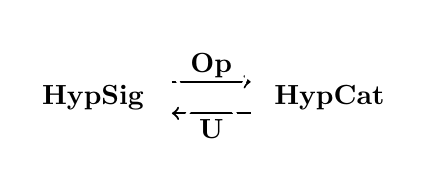
\begin{tikzpicture}[node distance={10mm}, thick, main/.style = {draw, circle, fill=black, inner sep=0pt, minimum width=2pt},
		letter/.style={circle,draw=white,very thick}] 
		
		
		\draw[->] (0,0.2) -- (1,0.2);
		\draw[->] (1,-0.2) -- (0,-0.2);

		
		\node[letter] (p) at (-1,0) {\textbf{HypSig}};
		\node[letter] (p) at (2,0) {\textbf{HypCat}};
		\node[letter] (p) at (.5,0.4) {\textbf{Op}};
		\node[letter] (p) at (.5,-0.4) {\textbf{U}};

	\end{tikzpicture}
	\end{center}
	donde \textbf{U} es el funtor olvidadizo de una hipergráfica a su signatura.

\end{prop}

\section{Lenguajes libres de contexto}

Sea $G$ signatura finita de hipergráfica. Consideremos sus objetos como símbolos, los nodos como reglas de producción y los morfismos en \textbf{Op}(G) como derivaciones, entonces obtenemos la noción de una gramática, más precisamente:

\begin{dfn}
	Un gramática operádica como una signatura finita de hipergráfica de la siguiente forma: 
	\[
		(B+V)^* \leftarrow G \to B
	\]
	donde $V$ es un vocabulario y $B$ es un conjunto de símbolos no terminales con un símbolo distinguido $s \in B$ y $G$ un conjunto de reglas de producciones. \\ El lenguaje generado por $G$ es: 
	\[
		\mathcal{L}(G) = \{ u \in V^*|\exists g: u \to s \in \textbf{Op}(G) \}
	\]
\end{dfn}

\nota{Agregar dos ejemplo. Lógica proposicional y del lenguaje}


Ahora, como anunciamos al inicio del capítulo, mostraremos la relación entre los lenguajes anteriores con la jerarquía de Chomsky. Para ello, veamos la siguientes definiciones y resultados.

\begin{dfn}
	
	Un gramática libre de contexto es una tupla $G=(V,B,P,s)$ donde $V$ es un vocabulario, $B$ es un conjunto de símbolos no terminales con un símbolo distinguido $s$ y $P$ es un conjunto de reglas de producción de la forma $A \to \alpha$ donde $A$ es un símbolo no terminal y $\alpha \in (V+B)^*$.\\
	Si $A \to \alpha$ es una regla de producción, para cualquier $\beta, \gamma \in (V+B)^*$ definimos la derivación 
	$\beta A \gamma \Rightarrow \beta \alpha \gamma$. 
	Consideramos $\Rightarrow ^*$ como la  cerradura transitiva de $\Rightarrow$. \\
	
	Definimos el lenguaje generado por $G$ como:
	
	$$ \mathcal{L}(G)= \{ w \in V^* | \exists s \Rightarrow w \} $$
	
	Decimos que un lenguaje $L$ es libre de contexto si existe una gramática $G$ libre de contexto tal que $L=L(G)$

\end{dfn}

Observemos que una oración en un lenguaje libre de contexto corresponde a una cadena en $V^*$ que puede ser derivada a partir de $s$ en $G$. \\

Ahora, la manera anterior de describir el lenguaje es eficiente para la generación de nuevas expresiones, sin embargo, puede no ser muy útil para el propósito de discriminar si una expresión dada pertenece, o no, al lenguaje. Con ese propósito surgen los árboles de derivación. 

\begin{dfn}
	
	Sea $G=(V,B,P,s)$ una gramática libre de contexto. \\
	Un árbol es un árbol de derivación para $G$ si:
	
	\begin{itemize}
		\item Cada vértice está etiquetado con un símbolo de $V \cup B \cup \{ \varepsilon \}$; 
		\item La raíz del árbol es $s$; 
		\item Si un vértice interior está etiquetado con A, entonces $A \in B$, es decir, no es un símbolo terminal. 
		\item Si un vértice $A$ tiene $n$ hijos, $A_1, \dots, A_n$, entonces:
		$$A \to A_1A_2 \cdots A_n$$
		
		es una regla de producción en $P$. \\
		\item Si un vértice está etiquetado con $\epsilon$, entonces es un hoja y, además, es el único hijo de su padre.
	\end{itemize}
	
	
\end{dfn}

Notemos que el diagrama del ejemplo uno corresponde a un árbol de derivación en la gramática $A \to \neg A | A \land A | A \lor A | A \to A | A \leftrightarrow A|a_0|a_1|a_2 $.\\ 
Con esto, podemos enunciar la siguiente proposición cuya prueba podemos consultar en \nota[ Agregar ref]. \\

\begin{prop}
	Sea $G=(V,B,P,s)$ una gramática libre de contexto. Entonces $s \Rightarrow ^* w$ si y sólo si existe un árbol de derivación para $G$ que produce a $w$. 
\end{prop}

Es fácil notar que un morfismo en un hipergráfica corresponde, de hecho, a un árbol de derivación. Con ello, tenemos el siguiente corolario:

\begin{thm}
	Sea $G$ una signatura de hipergráfica y $G'$ una gramática libre de contexto, entonces\\
	1. $L(G)$ es un lenguaje libre de contexto.\\
	2. Existe una signatura de hipergráfica que genera a $L(G')$. 
\end{thm}

\begin{proof}
	\nota{Pendiente.}
\end{proof}



\end{document}